We first introduce the datasets on which we conduct our experiments, and describe the experiment setup. We then describe our methodology for comparing the performance of various algorithms at the affiliation recommendation task. Finally, we discuss the results of experiments which apply the algorithms based on both the graph proximity model and the latent factors model in performing affiliation recommendation.

\subsection{Data}
We use two popular online social networks \textit{Orkut} and \textit{Youtube}, both operated by Google, for our experiments. The users of both the social networks explicitly identify themselves as belonging to some \textit{communities} or \textit{groups}. Thus, for each of the networks we have adjacency matrix $\A$ that identifies the memberships of the users in the groups and adjacency matrix $\SS$ that identifies friendships among users. For our experiments, we used data gathered by Mislove et al \cite{Mislove}. We compare the predictive ability of the algorithms using sub-networks extracted from these large networks \footnote{We extracted a small connected component from the large network for the propose of experimentation.}. The statistics for these networks are presented in Table \ref{tab:datasets}.

\begin{table}[h!]
\centering
\begin{tabular}{| l | r | r |} \hline
Feature & Orkut & Youtube\\ \hline
$N_{u}$ & 9123 & 16575 \\ \hline
$N_{g}$ & 75546 & 21326 \\ \hline
Average number of groups per user & 55.8 & 10.5\\ \hline
Minimum number of groups per user & 4 & 4\\ \hline
Mode of number of groups per user & 6 & 4\\ \hline
Average number of users per group & 6.7 & 8.1\\ \hline
Mode of number of users per group & 2 & 1 \\ \hline
Minimum number of users per group & 1 & 1\\ \hline
Average number of friends per user & 46 & 11.7\\ \hline
Mode of number of friends per user & 2 & 1\\ \hline
\end{tabular}
\caption{Details about the datasets used in experiments.}
\label{tab:datasets}
\end{table}

\subsection{Experiment setup}
For every user $u$, let $\E_u = \set{(u,v) \ | \ \A_{u,v} = 1}$ denote the affiliations of $u$, as observed in a given affiliation network $\A$. Invariably in all the experiments, we set aside a subset of these affiliations $\E_{u}^{(t)} \subset \E_u$ as test data (we use $|\E_u^{(t)}| = 30 \% |\E_u|$). The remaining affiliations $\E_u^{(tr)} = \E_u \setminus \E_u^{(t)}$ are used as training data for the recommendation algorithms.

All of our recommendation algorithms require ``learning'' parameters for some model of the affiliation process, and hence for the purposes of learning the parameters, we use a set of \textit{validation} edges $\E_u^{(v)} \subset \E_u^{(tr)}$ (we use $|\E_u^{(v)}| = 30 \% |\E_u^{(tr)}|$). During the validation process, we compare different model parameters based on the number of correct edges among $25 N_u$ recommendations \footnote{This is chosen because, in Section \ref{Evaluation method}, we argue that a predictive model should be judged based on the quality of its top few recommendations.} made using the model.

\subsubsection{Evaluation method}
\label{Evaluation method}
We now describe our methodology for evaluating the performance of an affiliation recommendation algorithm. We first introduce notions of interest, such as precision, sensitivity, specificity, ROC and AUC. We then describe the way in which we evaluate the performance of a recommendation algorithm based on its top 50 recommendations to the average user. We then demonstrate the importance of choosing the right evaluation method for the community recommendation task by showing that using a different, but less appropriate, evaluation strategy yields different results.

Three commonly used measures of quality of solutions in information retrieval and classification tasks are \textit{Precision}, \textit{Recall} or \textit{Sensitivity} and \textit{Specificity}. \textit{Precision} measures the exactness or fidelity of the prediction while \textit{Sensitivity} measures the completeness of the prediction. Suppose that the recommendation algorithm makes $n$ recommendations to a user. Then, \textit{Precision} is defined as the ratio of the number of correctly identified positives (true positives) to $n$, and \textit{Sensitivity} is the ratio of the number of correctly identified positives to the total number of positives i.e. $|\E_u^{(t)}|$. \textit{Specificity}, on the other hand, measures the ability of the recommender to exclude uninteresting affiliations from the recommendations it makes. It is defined as the fraction of such ``negative affiliations'' correctly excluded from the recommendation. All three of these performance measures range from 0 to 1.

Often, one is interested in evaluating the performance of a recommendation algorithm not for a single value of the number of recommendations $n$, but for the entire range of $n$. For a given recommendation algorithm and a user, sensitivity is a non-decreasing function of $n$, while specificity is a monotonically non-increasing function of $n$. The relationship between the increase in sensitivity, as $n$ increases, with the decrease in specificity is of interest in comparing the quality of recommendations. For a good recommendation, as $n$ increases, sensitivity increases without a big drop in specificity. The Reciever Operating Characteristics (ROC) curve, which is a plot of sensitivity vs (1 - specificity) for all values of $n$, is a common way of comparing the performance of classification algorithms over the entire range of $n$ (or equivalently cutoff scores). Area under the ROC curve, or AUC, is then used as a way to compare different classification algorithms: the greater the AUC, the better the algorithm's sensitivity vs 1-specificity tradeoff.

Consider a social network website, like Orkut or Facebook; or a vendor like Netflix which sells movies. They would be interested in making, let us say, five pages of recommendations to their users, but not much more than that: certainly not a hundred. Also, irrespective of whether a user participates in five communities or seventy, the social networking website would probably want to make roughly the same number of recommendations per user. So, we choose to evaluate the recommendation algorithms we propose based on their top 50 recommendations. We do this by examining a slice of the ROC curve formed by measuring the sensitivity and specificity the recommendation algorithm achieves for an average user at regular intervals between $n = 1$ and $n = 50$. To do this, for a given $n$, we compute the sensitivity and specificity for every user in the network, and take the mean of these values to be the average sensitivity and average specificity. We then plot the average sensitivity vs 1 - average specificity curve, as in Figure \ref{fig:summaryResults}. Note that comparisons made using this method are statistically robust, as the sensitivities and specificities of recommendation algorithms are averaged over, for example, 9500 users in Orkut and 16000 users in Youtube.

Let $k(n_u)$ be the number of ``good recommendations'' made by a recommendation algorithm for a user $u$, when it makes $n_u$ recommendations to that user. Then, the above ``per user'' sensitivity measure calculates $N_u^{-1} \sum_u \displaystyle\frac{k(n_u) }{|\E_u^{(t)}|}$. In our experiments, we will use $\forall u: n_u = 50$.

Contrast this with finding the ``global'' sensitivity $\dfrac{k'(n)}{\sum_u |\E_u^{(t)}|}$, where $k'(n)$ denotes the number of ``good recommendations'' made by a given recommendation algorithm while making $n$ predictions in total. For a fixed $n$, this ``global'' sensitivity is proportional to precision, and is a commonly used measure of performance of link prediction algorithms in the context of social network analysis. Note that, in this case, while $n = \sum_u n_u$, there is no guarantee that, for two given users $u$ and $v$, $n_u = n_v$; indeed the recommendation algorithm, when asked to make $n$ recommendations, may not make any recommendations at all for some users. Therefore, this measure of goodness of a recommendation algorithm is not equivalent to the ``per user'' sensitivity described earlier.

Also, judging identical algorithms on identical datasets, using this alternate evaluation method can yield very different rankings of recommendation algorithms, as illustrated by comparing Figure \ref{fig:linkPredictionEvaluation} with Figure \ref{fig:summaryResults}. Hence, the choice of an appropriate method for evaluating affiliation recommendations is an important one. 

\begin{figure}[h]
  \begin{center}
    \subfigure[Orkut dataset]{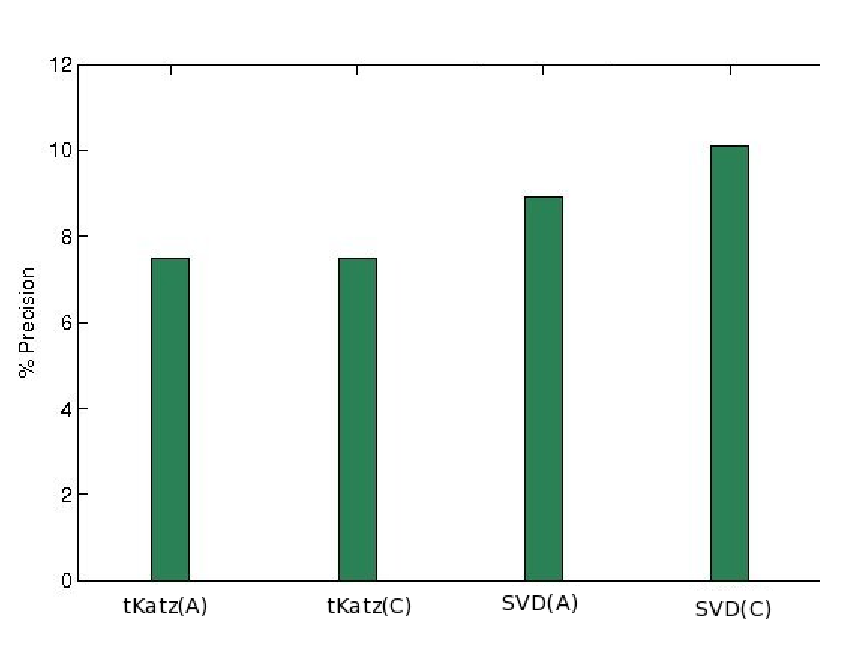
\includegraphics[scale=0.5]{OrkutLinkPredictionEvaluation.eps}}
    \subfigure[Youtube dataset]{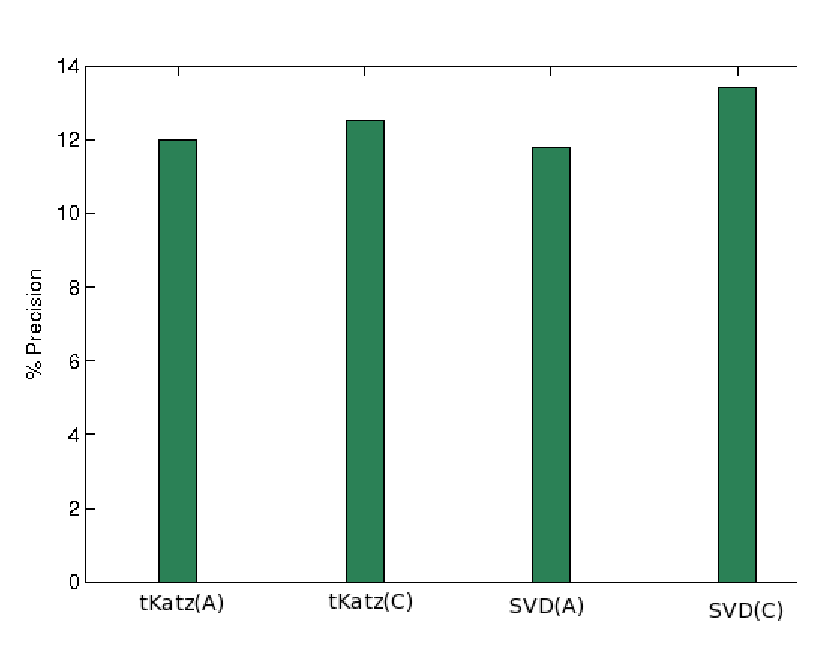
\includegraphics[scale=0.5]{YoutubeLinkPredictionEvaluation.eps}}
  \end{center}
  \caption{Comparison of recommendation algorithms using ``global sensitivity'' yields results different from Figure \ref{fig:summaryResults} while making $\sum_u E_u$ recommendations in total (See Section \ref{Evaluation method}).}
  \label{fig:linkPredictionEvaluation}
\end{figure}

\begin{figure}[h]
  \begin{center}
    \subfigure[Orkut dataset]{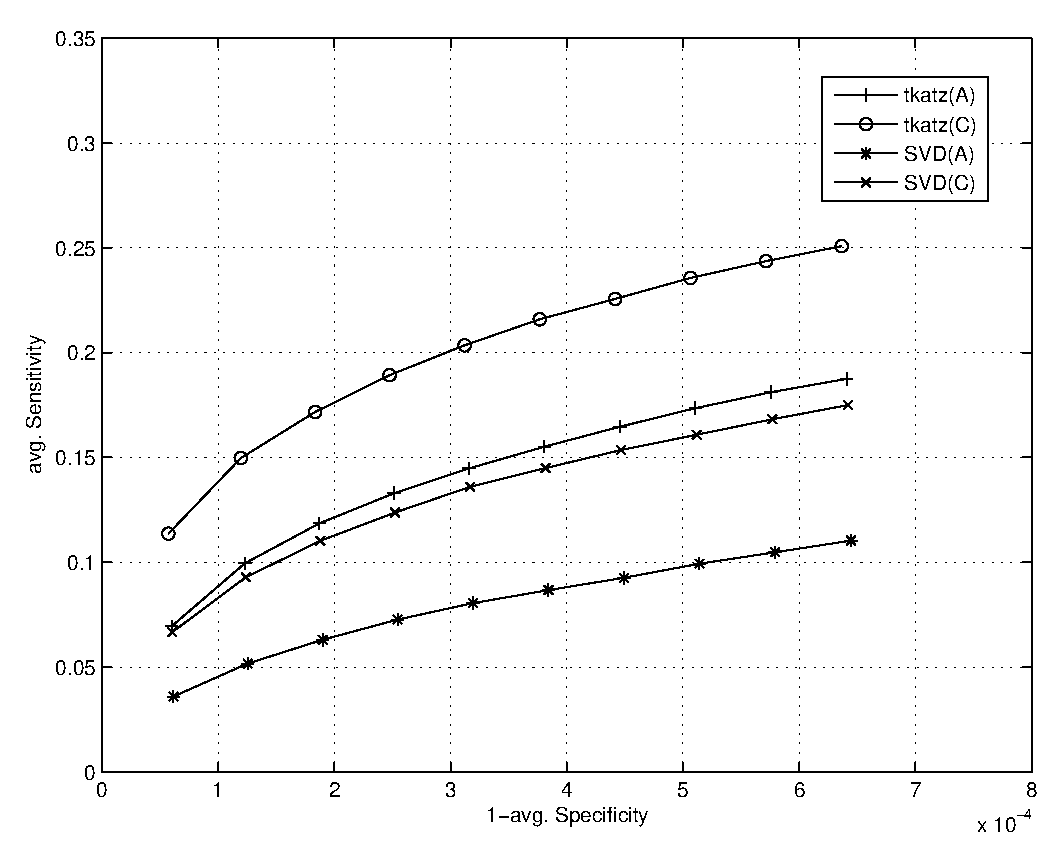
\includegraphics[scale=0.4]{summaryOrkut.eps}}
    \subfigure[Youtube dataset]{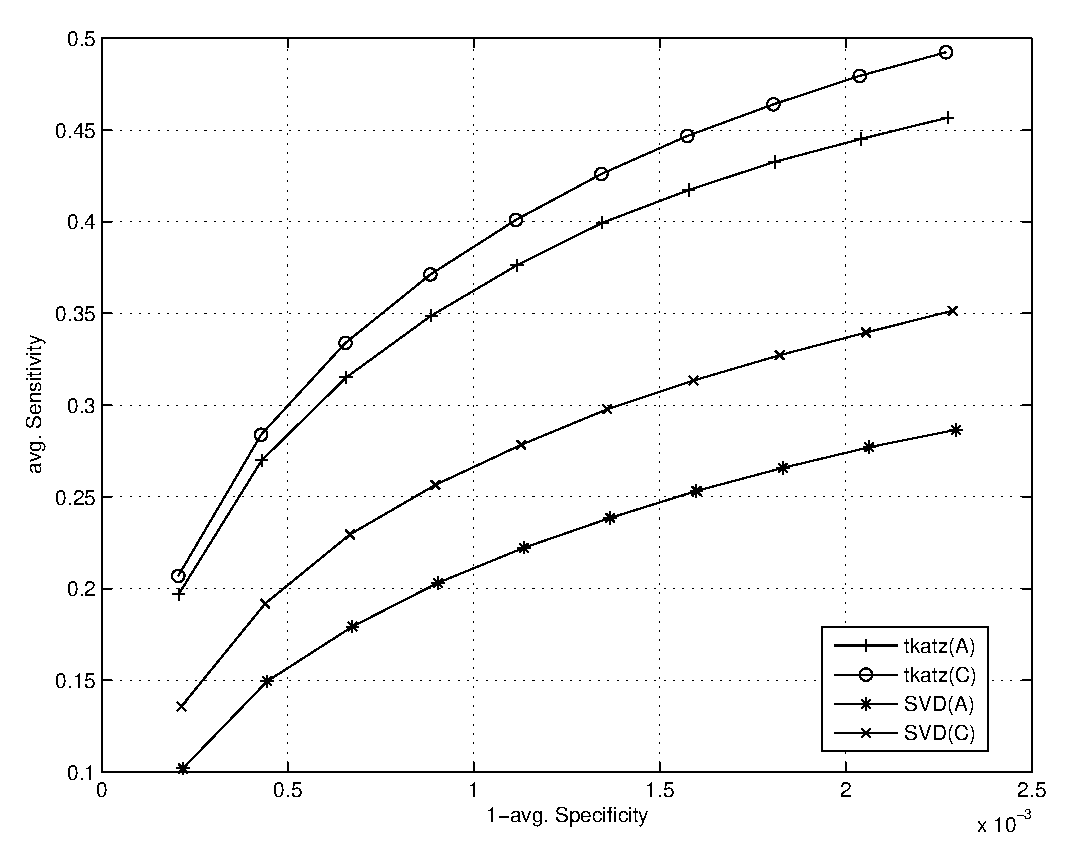
\includegraphics[scale=0.4]{summaryYoutube.eps}}
  \end{center}
  \caption{Comparison of recommendation algorithms based on graph proximity and latent factors models, as described in Section \ref{Evaluation method}. The leading slice of the ROC curve is shown. The graph proximity based predictors consistently outperform latent factors based predictors in the two datasets. See Section \ref{Results and Discussion} for discussion.}
  \label{fig:summaryResults}
\end{figure}

\begin{figure}[h]
  \begin{center}
    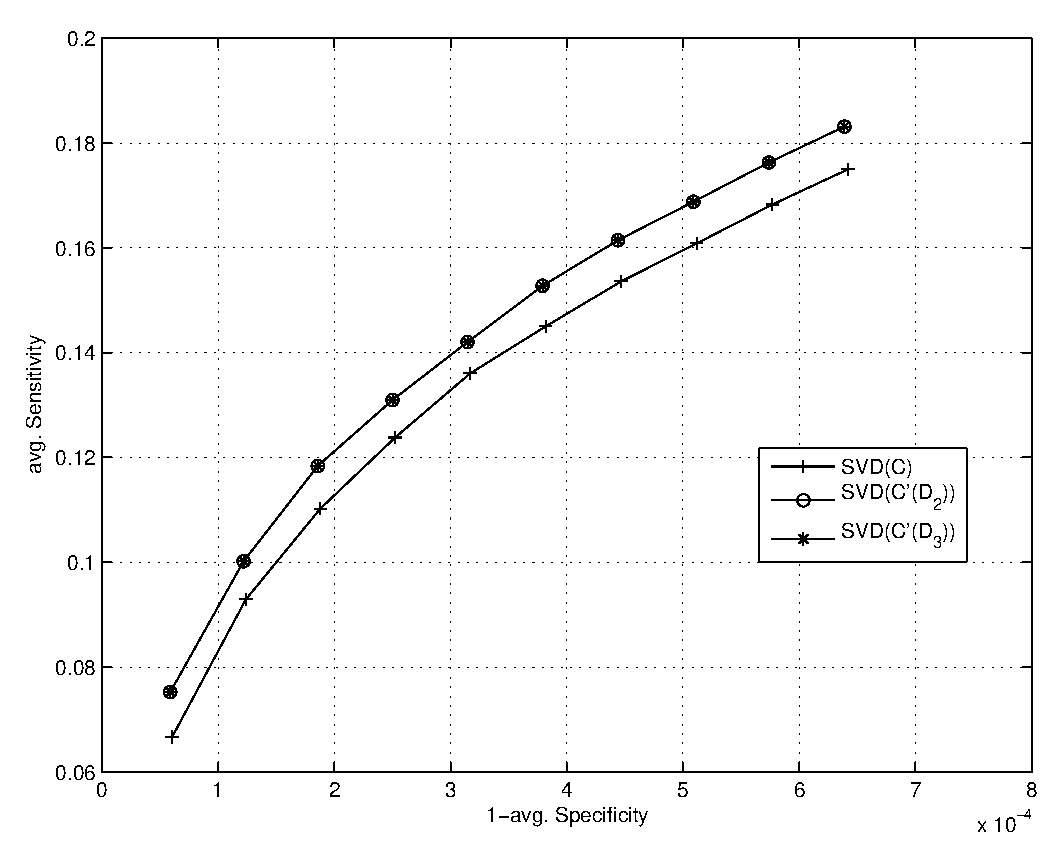
\includegraphics[scale=0.4]{summarySVDOrkut.eps}
  \end{center}
  \caption{Comparison of latent factors based algorithms for various choices of $\D$, for the Orkut dataset. See Section \ref{Results and Discussion} for discussion.}
  \label{fig:summarySVD}
\end{figure}

\subsection{Results and Discussion}
\label{Results and Discussion}
In this section, we report and analyse the performance of the various recommendation algorithms, based on the graph proximity model and latent factors model discussed in Section \ref{Models}. We compare the performance of the graph proximity based methods with latent factors based methods based on the average sensitivity and average specificity metrics introduced earlier, for a given number of recommendations in the range [5,50] (in steps of 5).

The results are reported in Figure \ref{fig:summaryResults}.
Consider the performance of the recommendation algorithms on the Orkut dataset in Figure \ref{fig:summaryResults} (a). SVD($\A$) gives the lowest performance of all the methods. SVD($\C$) performs better than SVD($\A$), which is expected given that it uses information from the friendship network $\SS$ in addition to the information from affiliation network $\A$. For the average user, the graph proximity model based methods significantly outperform latent factors based methods as observed from the figure. In particular, we see that tKatz($\C$) performs much better than tKatz($\A$), which in turn outperforms latent factor based methods. We see that the information in the friendship network indeed proves highly beneficial to making affiliation recommendations and graph proximity based methods exploit this information the most.

Another interesting comparison of latent factor methods based on the choice of $\D$ in constructing the combined network $\C'$ given in (\ref{e:generalizedCombined}), is presented in Figure \ref{fig:summarySVD}. We observe that the choice of $\D$ does not appear to make any significant difference in the performance of the recommendation algorithm. In the plot, $\D_2$ denotes using $\A^{T}\A$ for $\D$ in $\C'$  while $\D_3$ denotes using $\lambda \A^{T}\A$, where $\lambda$ is also the weight associated with $\SS$ in the combined graph. Though, in case of the Orkut dataset, we see that SVD($\C', \D$) performs slightly better than SVD($\C$), the choice of $\D \neq 0$ does not affect the performance. In case of Youtube (plots not shown), our experiments indicate that $\D$ is not useful at all. The potential choices for $\D$ do not perform any better than $\D = 0$.

The summary of performances of the algorithms on the Youtube dataset is shown in Figure \ref{fig:summaryResults} (b). We observe that the case for Youtube is similar to that of Orkut, in that graph proximity based algorithms significantly outperform latent factors based algorithms. In particular, tKatz($\C$) is highly successful compared to the other methods. 

The best parameters learnt by the various algorithms are presented in Table \ref{tab:parameters}. Note that the best parameter $\beta = 10^{-12}$ implies that the calculated tKatz measure was effectively using the common neighbors method. In other words, users and communities connected by path lengths 5 or more are not useful in making affiliation recommendations.

\begin{table}[h!]
\centering
\begin{tabular}{| c | p{2.4cm} | p{2.4cm} |} \hline
Algorithm&Orkut&Youtube\\ \hline
SVD($\C$) & $d=50, \gl = 0.8$ & $d = 90, \gl = 1$ \\ \hline
SVD($\C'(\lambda \A^{T} \A)$) & $d = 60, \gl = 0.6$ & $d = 70, \gl = 1$ \\ \hline
tKatz($\A$) & $\gb = 10^{-12}$ & $\gb = 10^{-12}$ \\ \hline
tKatz($\C$) & $\gb = 0.01, \gl = 0.2$ & $\gb = 0.1, \gl = 0.4$ \\ \hline
\end{tabular}
\caption{Best parameters learned by the recommendation algorithms using validation.}
\label{tab:parameters}
\end{table}

We see that the recommendation algorithms perform consistently across the two datasets, and the evaluations are robust as the specificities and sensitivities are averaged over 9000 users in Orkut and 16000 users in Youtube.
